\documentclass[
11pt, % The default document font size, options: 10pt, 11pt, 12pt
%codirector, % Uncomment to add a codirector to the title page
]{charter} 


% El títulos de la memoria, se usa en la carátula y se puede usar el cualquier lugar del documento con el comando \ttitle
\titulo{Entrenamiento de robot caminante por imitación y RL usando ZMP como generador de datos de referencia} 

% Nombre del posgrado, se usa en la carátula y se puede usar el cualquier lugar del documento con el comando \degreename
%\posgrado{Carrera de Especialización en Sistemas Embebidos} 
%\posgrado{Carrera de Especialización en Internet de las Cosas} 
\posgrado{Carrera de Especialización en Inteligencia Artificial}
%\posgrado{Maestría en Sistemas Embebidos} 
%\posgrado{Maestría en Internet de las cosas}

% Tu nombre, se puede usar el cualquier lugar del documento con el comando \authorname
% IMPORTANTE: no omitir titulaciones ni tildación en los nombres, también se recomienda escribir los nombres completos (tal cual los tienen en su documento)
\autor{Ing. Francisco Antonio Cofré Villalón}

% El nombre del director y co-director, se puede usar el cualquier lugar del documento con el comando \supname y \cosupname y \pertesupname y \pertecosupname
\director{Título y Nombre del director}
\pertenenciaDirector{pertenencia} 
\codirector{} % para que aparezca en la portada se debe descomentar la opción codirector en los parámetros de documentclass
\pertenenciaCoDirector{FIUBA}

% Nombre del cliente, quien va a aprobar los resultados del proyecto, se puede usar con el comando \clientename y \empclientename
\cliente{Nombre del cliente}
\empresaCliente{Empresa del cliente}
 
\fechaINICIO{21 de octubre de 2025}		%Fecha de inicio de la cursada de GdP \fechaInicioName
\fechaFINALPlan{9 de diciembre de 2025} 	%Fecha de final de cursada de GdP
\fechaFINALTrabajo{junio de 2026}	%Fecha de defensa pública del trabajo final


\begin{document}

\maketitle
\thispagestyle{empty}
\pagebreak


\thispagestyle{empty}
{\setlength{\parskip}{0pt}
\tableofcontents{}
}
\pagebreak


\section*{Registros de cambios}
\label{sec:registro}


\begin{table}[ht]
\label{tab:registro}
\centering
\begin{tabularx}{\linewidth}{@{}|c|X|c|@{}}
\hline
\rowcolor[HTML]{C0C0C0} 
Revisión & \multicolumn{1}{c|}{\cellcolor[HTML]{C0C0C0}Detalles de los cambios realizados} & Fecha      \\ \hline
0      & Creación del documento                                 &\fechaInicioName \\ \hline
1      & Se completa hasta el punto 5 inclusive                & {5} de {noviembre} de 2025 \\ \hline
2      & Se completa hasta el punto 9 inclusive
%		  Se puede agregar algo más \newline
%		  En distintas líneas \newline
		                                                      & {12} de {noviembre} de 2025 \\ \hline
3      & Se completa hasta el punto 12 inclusive                & {23} de {noviembre} de 2025 \\ \hline
4      & Se completa el plan	                                 & {30} de {noviembre} de 2025 \\ \hline

% Si hay más correcciones pasada la versión 4 también se deben especificar acá

\end{tabularx}
\end{table}

\pagebreak



\section*{Acta de constitución del proyecto}
\label{sec:acta}

\begin{flushright}
Buenos Aires, \fechaInicioName
\end{flushright}

\vspace{2cm}

Por medio de la presente se acuerda con el \authorname\hspace{1px} que su Trabajo Final de la \degreename\hspace{1px} se titulará ``\ttitle'' y consistirá en la simulación de un robot caminante y el entrenamiento de las políticas de control de su marcha aplicando aprendizaje por refuerzo. El trabajo tendrá un presupuesto preliminar estimado de \textcolor{red}{600} horas y un costo estimado de \textcolor{red}{\$ XXX}, con fecha de inicio el \fechaInicioName\hspace{1px} y fecha de presentación pública en \textcolor{red}{\fechaFinalName}.

Se adjunta a esta acta la planificación inicial.

\vfill

% Esta parte se construye sola con la información que hayan cargado en el preámbulo del documento y no debe modificarla
\begin{table}[ht]
\centering
\begin{tabular}{ccc}
\begin{tabular}[c]{@{}c@{}}Dr. Ing. Ariel Lutenberg \\ Director posgrado FIUBA\end{tabular} & \hspace{2cm} & \begin{tabular}[c]{@{}c@{}}\clientename \\ \empclientename \end{tabular} \vspace{2.5cm} \\ 
\multicolumn{3}{c}{\begin{tabular}[c]{@{}c@{}} \supname \\ Director del Trabajo Final\end{tabular}} \vspace{2.5cm} \\
\end{tabular}
\end{table}




\section{1. Descripción técnica-conceptual del proyecto a realizar}
\label{sec:descripcion}



El proyecto consiste en diseñar y entrenar en simulación un sistema de desplazamiento para un robot caminante destinado a realizar tareas en obras de construcción. El objetivo técnico es obtener una política de control de la marcha capaz de andar de forma estable frente a perturbaciones, mientras que el objetivo de negocio es explorar tecnologías que, en una etapa posterior, permitan automatizar tareas físicamente exigentes y peligrosas de una empresa constructora.

Como consecuencia de terrenos irregulares, cambios diarios en el entorno, obstáculos imprevistos, desniveles y riesgo de caídas, la automatización ha avanzado más lentamente en el sector de la construcción. Muchos procesos que requieren desplazamiento y manipulación en estos entornos son difíciles de automatizar con métodos tradicionales de control. Sin embargo, a mayor nivel de automatización de tareas repetitivas, mayor es el potencial de reducir costos para los clientes finales sin sacrificar calidad, además de disminuir la exposición de los operarios a condiciones peligrosas.

Este proyecto utiliza el ZMP (Zero Moment Point) como generador de datos de referencia. El ZMP es un criterio de estabilidad: si el punto donde la resultante de las fuerzas de reacción del suelo tiene un momento nulo (el ZMP) permanece dentro del polígono de apoyo, se garantiza la estabilidad en superficies planas. Proporciona una condición suficiente de estabilidad y permite el cálculo de trayectorias expertas de forma determinista, pero es inadecuado frente a perturbaciones externas y es energéticamente ineficiente.

El estado del arte combina aprendizaje profundo y aprendizaje por refuerzo (DRL) desde cero. Aquí el agente puede descubrir autónomamente estrategias de control a través de prueba y error, y adaptarse a escenarios imprevistos, pero es computacionalmente costoso.

Como se observa en la figura \ref{fig:diagBloques}, no se utiliza ZMP como controlador final, sino como un generador de datos de referencia, o de demostraciones expertas para iniciar la política de RL. Esto puede reducir el costo de la exploración aleatoria inicial. El agente no empieza ciego, sino que ya sabe cómo caminar de forma estable, luego el RL se utiliza solo para robustecer el comportamiento ante posibles perturbaciones.


\begin{figure}[htpb]
\centering 
\includegraphics[width=.5\textwidth]{./Figuras/diagBloques.png}
\caption{Diagrama en bloques del sistema.}
\label{fig:diagBloques}
\end{figure}

\vspace{25px}




\section{2. Identificación y análisis de los interesados}
\label{sec:interesados}





% Please add the following required packages to your document preamble:
% \usepackage[table,xcdraw]{xcolor}
% Beamer presentation requires \usepackage{colortbl} instead of \usepackage[table,xcdraw]{xcolor}

\begin{table}[H]
\begin{tabular}{|l|l|l|l|}
\hline
\rowcolor[HTML]{C0C0C0} 
Rol           & Nombre y Apellido                                                               & Organización                   & Puesto                     \\ \hline
Cliente       & \clientename                                                     & \empclientename & -                          \\ \hline
Responsable   & \begin{tabular}[c]{@{}l@{}}Ing. Francisco Antonio\\ Cofré Villalón\end{tabular} & FIUBA                          & Alumno                     \\ \hline

Orientador    & \supname                                                         & \pertesupname   & Director del Trabajo Final \\ \hline



\end{tabular}
\end{table}

\section{3. Propósito del proyecto}
\label{sec:proposito}


El problema que abordará el proyecto es la automatización en entornos difíciles de predecir. A diferencia de una planta industrial, un sitio de construcción es dinámico, caracterizado por terreno irregular, escombros, obstáculos imprevistos y la necesidad de navegar en múltiples niveles. Este dominio de problema justifica el enfoque del proyecto en la locomoción bípeda. Soluciones robóticas más simples, como las plataformas con ruedas o los brazos robóticos estacionarios, son inadecuadas para la navegación y movilidad requeridas.


\section{4. Alcance del proyecto}
\label{sec:alcance}








El proyecto incluye:
\begin{itemize}
	\item El diseño de un modelo 3D del robot bípedo.
	\item La configuración de un entorno de simulación física que modele la dinámica, las colisiones y las fuerzas de reacción del suelo.
	\item El algoritmo de generación de trayectorias basado en el Zero Moment Point (ZMP) y el registro de las demostraciones (estados, acciones) generadas en la simulación.
	\item Código necesario para el entrenamiento de la política.
	\item Pruebas para validar la política de locomoción final.
	
\end{itemize}

El proyecto no incluye:
\begin{itemize}
	\item El diseño, fabricación o costo de componentes.
	\item La simulación del torso, brazos y manos.
	\item La transferencia de la política a un robot físico.
    
\end{itemize}


\section{5. Supuestos del proyecto}
\label{sec:supuestos}


Para el desarrollo del presente proyecto se supone que:

\begin{itemize}
	\item Se dispondrá de suficientes horas semanales para cumplir el cronograma estimado del proyecto y completar las aproximadamente 600 horas totales previstas.
	
	\item NVIDIA Isaac Sim, Isaac Lab, PyTorch y los frameworks de RL utilizados permanecerán disponibles durante toda la duración del proyecto, sin cambios de licencia ni compatibilidad.
	
	\item Se asume que el simulador podrá representar de manera suficientemente realista la dinámica del robot, los contactos y las fuerzas del suelo como para producir datos útiles para IL y RL.
	
	\item Se asume que el diseño del robot y su modelo 3D podrán integrarse sin errores graves al entorno de simulación.
	
	\item La disponibilidad del tiempo de cómputo será suficiente para las múltiples iteraciones requeridas por el entrenamiento de las políticas de IL y RL en el entorno de simulación física.
	
	\item Se contará con suficiente memoria para ejecutar simulaciones físicas y entrenar modelos de IL y RL sin bloqueos críticos.
    
\end{itemize}


\section{6. Product Backlog}
\label{sec:backlog}




Para obtener los Story Points (SP) de cada historia de usuario se evalúan tres factores:

Dificultad (D): cantidad de trabajo estimado.

Complejidad (C): nivel técnico requerido.

Incertidumbre (I): grado de riesgo o novedad.

Cada dimensión se puntúa en una escala de uno a diez, se suman y luego se redondea hacia el número superior más próximo de la serie de Fibonacci:

1, 2, 3, 5, 8, 13, 21, 34…


\begin{itemize}
  \item \textbf{\'{E}pica 1: Modelo 3D y entorno de simulación}
    \begin{itemize}
      \item HU1: Como responsable de simulación, quiero un modelo 3D del robot bípedo para poder ajustar dimensiones, masas, calcular trayectorias y entrenar agentes.
      \item D: 3, C: 3, I: 3, SP: 13.
      \item HU2: Como responsable de simulación, quiero un entorno de simulación para calcular trayectorias y entrenar agentes.
      \item D: 3, C: 3, I: 3, SP: 13.
    \end{itemize}
  \item \textbf{\'{E}pica 2: Generación de trayectorias expertas con ZMP}
    \begin{itemize}
      \item HU3: Como responsable de control, quiero que el sistema genere trayectorias de marcha estables usando ZMP para poder utilizarlas como demostraciones expertas en el entrenamiento por imitación.
      \item D: 3, C: 3, I: 3, SP: 13.
      \item HU4: Como responsable de control, quiero poder ver indicados el ZMP, el centro de masa y los contactos con el suelo durante la marcha para confirmar que las trayectorias cumplen las condiciones de estabilidad.
      \item D: 3, C: 3, I: 3, SP: 13.
    \end{itemize}
  \item \textbf{\'{E}pica 3: Entrenamiento por imitación y RL de la marcha bípeda}
    \begin{itemize}
      \item HU5: Como responsable de ML, quiero entrenar una política inicial a partir de las demostraciones generadas con ZMP para obtener un caminante estable en pocas iteraciones.
      \item D: 3, C: 3, I: 3, SP: 13.
      \item HU6: Como responsable de ML, quiero mejorar la rapidez, definida como la distancia recorrida en simulación dividida por el tiempo transcurrido en simulación, y la estabilidad frente a perturbaciones, definida como la razón entre caídas causadas por perturbaciones y el número total de perturbaciones aplicadas, utilizando RL.
      
      \item D: 3, C: 3, I: 3, SP: 13.
    \end{itemize}
  \item \textbf{\'{E}pica 4: Experimentación y análisis de resultados}
    \begin{itemize}
      \item HU7: Como responsable de ML, quiero evaluar el progreso de la política para medir la mejora del agente durante el entrenamiento.
      \item D: 3, C: 3, I: 3, SP: 13.
      \item HU8: Como responsable de ML, quiero ver gráficos que resuman la estabilidad, rapidez y que comparen ZMP e IL+RL.
      \item D: 3, C: 3, I: 3, SP: 13.
    \end{itemize}
\end{itemize}


\section{7. Criterios de aceptación de historias de usuario}
\label{sec:criteriosAceptacion}



\begin{itemize}
  \item \textbf{\'{E}pica 1: Modelo 3D y entorno de simulación}
    \begin{itemize}
      \item HU1: URDF/USD con articulaciones (cadera, rodilla, tobillo) y masa superior. El modelo se exporta e integra sin errores en el entorno de simulación seleccionado. En una prueba estática, el robot se mantiene de pie.

      \item HU2: El mundo simula contacto, fricción y colisión. Se pueden salvar y reproducir series de acciones.
    \end{itemize}
  \item \textbf{\'{E}pica 2: Generación de trayectorias expertas con ZMP}
    \begin{itemize}
      \item HU3: Generador de trayectorias funciona. Se exporta dataset con N pasos. Dataset se puede cargar sin errores.
      \item HU4: Se muestra polígono de soporte, centro de masa y ZMP en tiempo real.
    \end{itemize}
  \item \textbf{\'{E}pica 3: Entrenamiento por imitación y RL de la marcha bípeda}
    \begin{itemize}
      \item HU5: Entrena política inicial. Logra caminar X metros sin caídas en entorno base. Secuencia es reproducible.
      \item HU6: Supera la política inicial en caídas, rapidez y energía dividida por distancia.
    \end{itemize}
  \item \textbf{\'{E}pica 4: Experimentación y análisis de resultados}
    \begin{itemize}
      \item HU7: Pruebas de tasa de caídas, velocidad, trayectorias CoM/ZMP, energía/distancia. Pruebas con perturbaciones, rugosidad, obstáculos.
      \item HU8: Metodología, registros, videos, gráficos.
    \end{itemize}
\end{itemize}

%\textbf{Reglas para definir criterios de aceptación:}
%\begin{itemize}
  %\item Medibles y verificables.
  %\item Especificar cuándo una historia se considera completada.
  %\item Incluir condiciones específicas.
  %\item No ambiguos.
 % \item Probables de testear funcional o técnicamente.
 % \item Mínimo 3 criterios por HU.
%\end{itemize}

\section{8. Fases de CRISP-DM}

De acuerdo con la metodología CRISP-DM, el desarrollo del proyecto se organizará en las siguientes fases:


\begin{enumerate}
  \item \textbf{Comprensión del negocio:} En esta etapa se analiza el problema de movilidad autónoma en obras de construcción, identificando actores, restricciones y objetivos de valor para la empresa constructora. Se define con claridad el objetivo del proyecto (obtener una política de marcha estable y robusta en simulación) y los criterios de éxito tanto técnicos (estabilidad, velocidad, eficiencia energética) como de negocio (potencial reducción de riesgos operativos y de costos en futuros desarrollos robóticos).
  
  \item \textbf{Comprensión de los datos:} Aquí se estudian en detalle las fuentes de datos disponibles en el simulador: estados del robot, fuerzas de contacto, trayectorias generadas con ZMP y registros de episodios de entrenamiento. Se evalúan su calidad, volumen, cobertura de escenarios y posibles sesgos, verificando que resulten adecuados para entrenar políticas mediante aprendizaje por imitación (IL) y aprendizaje por refuerzo (RL).
  
  \item \textbf{Preparación de los datos:} En esta fase se construye el conjunto de demostraciones expertas a partir de las trayectorias ZMP y se generan los conjuntos de episodios para RL. Se realizan tareas de selección de variables (posiciones, velocidades, fuerzas relevantes), limpieza de registros, normalización de magnitudes, etiquetado de eventos (caídas, perturbaciones) y particionado en conjuntos de entrenamiento, validación y prueba, de modo de asegurar datos consistentes para el modelado.
  
  \item \textbf{Modelado:} A partir de los datos preparados se diseñan e implementan los modelos de control: la política inicial obtenida por aprendizaje por imitación y la política refinada mediante aprendizaje por refuerzo. Esta fase incluye la elección de arquitecturas de redes neuronales, el diseño de la función de recompensa, la selección de algoritmos específicos de RL y la definición de los hiperparámetros clave del entrenamiento, considerando el compromiso entre desempeño y complejidad computacional.
  
  \item \textbf{Evaluación del modelo:} En esta etapa se analiza el desempeño de las políticas entrenadas mediante métricas cuantitativas: distancia recorrida sin caídas, velocidad media, energía consumida por unidad de distancia y tasas de caídas ante perturbaciones y variaciones del terreno. Se comparan sistemáticamente los resultados del controlador basado en ZMP frente a las políticas IL+RL y se revisa si las prestaciones alcanzadas se encuentran en un rango razonable respecto del estado del arte reportado en la literatura. Cuando los resultados no cumplen los criterios de éxito, se retroalimenta el proceso revisando fases previas de preparación de datos o modelado.
  
  \item \textbf{Despliegue:} Aunque el proyecto se limita a la simulación, la última fase es la documentación del entorno, de los modelos entrenados y la provisión de código para entrenamiento y evaluación. Esto permitirá que otros investigadores puedan replicar los experimentos, extender la simulación a nuevos escenarios, entrenar la parte superior del robot y, en etapas posteriores, la transferencia de las políticas a un prototipo físico.
  
\end{enumerate}


\section{9. Desglose del trabajo en tareas}
\label{sec:wbs}

\begin{table}[htpb]
\centering
\begin{tabularx}{\linewidth}{@{}|c|X|c|c|@{}}
\hline
\rowcolor[HTML]{C0C0C0} %una semana para buscar info
Historia de usuario & Tarea técnica & Estimación & Prioridad \\ \hline
HU1 & Determinar y especificar componentes. & 6 h & Alta \\ \hline
HU1 & Modelo 3D sensores actuadores vínculos (URDF/USD). & 8 h & Alta \\ \hline
HU2 & Configurar una escena base en simulador. & 5 h & Media \\ \hline
HU2 & Cargar y validar robot en simulador. & 6 h & Alta \\ \hline
HU3 & Calcular ZMP.  & 6 h & Alta \\ \hline
HU3 & Implementar el generador de trayectorias. & 8 h & Alta \\ \hline
HU4 & Mostrar ZMP, centro de masa y sus trayectorias en la simulación. & 5 h & Media \\ \hline
HU4 & Mostrar polígono de apoyo en la simulación. & 6 h & Alta \\ \hline
HU5 & Entrenar la política por imitación con el dataset de demostraciones. & 6 h & Alta \\ \hline
HU5 & Integrar la política entrenada en el simulador. & 8 h & Alta \\ \hline
HU6 & Configurar y ejecutar el algoritmo de RL elegido. & 5 h & Media \\ \hline
HU6 & Irregularidades, cambios de velocidad objetivo. & 6 h & Alta \\ \hline
HU7 & Registrar evolución de métricas.  & 6 h & Alta \\ \hline
HU7 & Automatizar registro y almacenamiento de métricas y logs. & 8 h & Alta \\ \hline
HU8 & Definir escenarios, perturbaciones, métricas y formato de registros y videos. & 5 h & Media \\ \hline
HU8 & Implementar notebooks generen gráficos de estabilidad y rapidez, y que comparen ZMP e IL+RL. & 6 h & Alta \\ \hline
\end{tabularx}
\end{table}


\vspace{1cm}



\section{10. Planificación de Sprints}
\begin{table}[htpb]
\centering
% \caption{Formato sugerido}
\begin{tabularx}{\linewidth}{@{}|l|l|X|c|l|c|@{}}
\hline
\rowcolor[HTML]{C0C0C0}
Sprint & HU o fase & Tarea & SP & Responsable & \% Completado \\ \hline
Sprint 0 & Planificación & Definir alcance y cronograma. & 10 h & Alumno & X\% \\ \hline
Sprint 0 & Planificación & Reunión con el tutor/cliente. & 5 h & Alumno & X\% \\ \hline
Sprint 0 & Planificación & Ajuste de los entregables. & 6 h & Alumno & X\% \\ \hline
Sprint 1 & HU1 & Determinar y especificar componentes, parámetros físicos y sensores. & 6 h / 3 SP & Alumno & 0\% \\ \hline
Sprint 1 & HU1 & Modelo 3D con sensores, actuadores y vínculos (URDF/USD). & 10 h / 5 SP & Alumno & 0\% \\ \hline
Sprint 2 & HU2 & Configurar una escena base en el simulador (mundo, gravedad, suelo). & 7 h / 5 SP & Alumno & 0\% \\ \hline
Sprint 2 & HU2 & Cargar y validar el robot bípedo en el simulador. & 10 h / 5 SP & Alumno & 0\% \\ \hline
Sprint 3 & HU3 & Implementar cálculo del ZMP a partir de fuerzas de contacto. & 7 h / 5 SP & Alumno & 0\% \\ \hline
Sprint 3 & HU3 & Implementar el generador de trayectorias de marcha basadas en ZMP. & 10 h / 5 SP & Alumno & 0\% \\ \hline
Sprint 4 & HU4 & Visualizar ZMP, polígono de soporte y centro de masa en tiempo real. & 7 h / 5 SP & Alumno & 0\% \\ \hline
\end{tabularx}
\end{table}


\begin{table}[htpb]
\centering
% \caption{Formato sugerido}
\begin{tabularx}{\linewidth}{@{}|l|l|X|c|l|c|@{}}
\hline
\rowcolor[HTML]{C0C0C0}
Sprint & HU o fase & Tarea & SP & Responsable & \% Completado \\ \hline


Sprint 4 & HU4 & Integrar visualización en la escena de simulación ya configurada. & 10 h / 5 SP & Alumno & 0\% \\ \hline
Sprint 5 & HU5 & Entrenar la política inicial por imitación (behavior cloning). & 7 h / 5 SP & Alumno & 0\% \\ \hline
Sprint 5 & HU5 & Integrar la política entrenada en el simulador y validar marcha base. & 10 h / 5 SP & Alumno & 0\% \\ \hline
Sprint 6 & HU6 & Configurar y ejecutar el algoritmo de RL elegido. & 7 h / 5 SP & Alumno & 0\% \\ \hline
Sprint 6 & HU6 & Entrenar robustez a irregularidades y cambios de velocidad objetivo. & 10 h / 5 SP & Alumno & 0\% \\ \hline
Sprint 7 & HU7 & Diseñar y registrar métricas (caídas, velocidad, energía/distancia). & 7 h / 5 SP & Alumno & 0\% \\ \hline
Sprint 7 & HU7 & Automatizar registro y almacenamiento de métricas. y logs & 10 h / 5 SP & Alumno & 0\% \\ \hline
Sprint 8 & HU8 & Desarrollar notebooks para generación de gráficos y tablas. & 7 h / 5 SP & Alumno & 0\% \\ \hline
Sprint 8 & HU8 & Integrar dashboards/notebooks en el flujo de experimentación. & 10 h / 5 SP & Alumno & 0\% \\ \hline
Sprint 9 & Escritura & Redacción memoria. & 50 h / 34 SP & Alumno & 0\% \\ \hline
Sprint 10 & Defensa & Preparación de la exposición. & 20 h / 13 SP & Alumno & 0\% \\ \hline
\end{tabularx}
\end{table}



\section{11. Diagrama de Gantt (sprints)}
\label{sec:gantt}




\begin{figure}[htpb]
\centering 
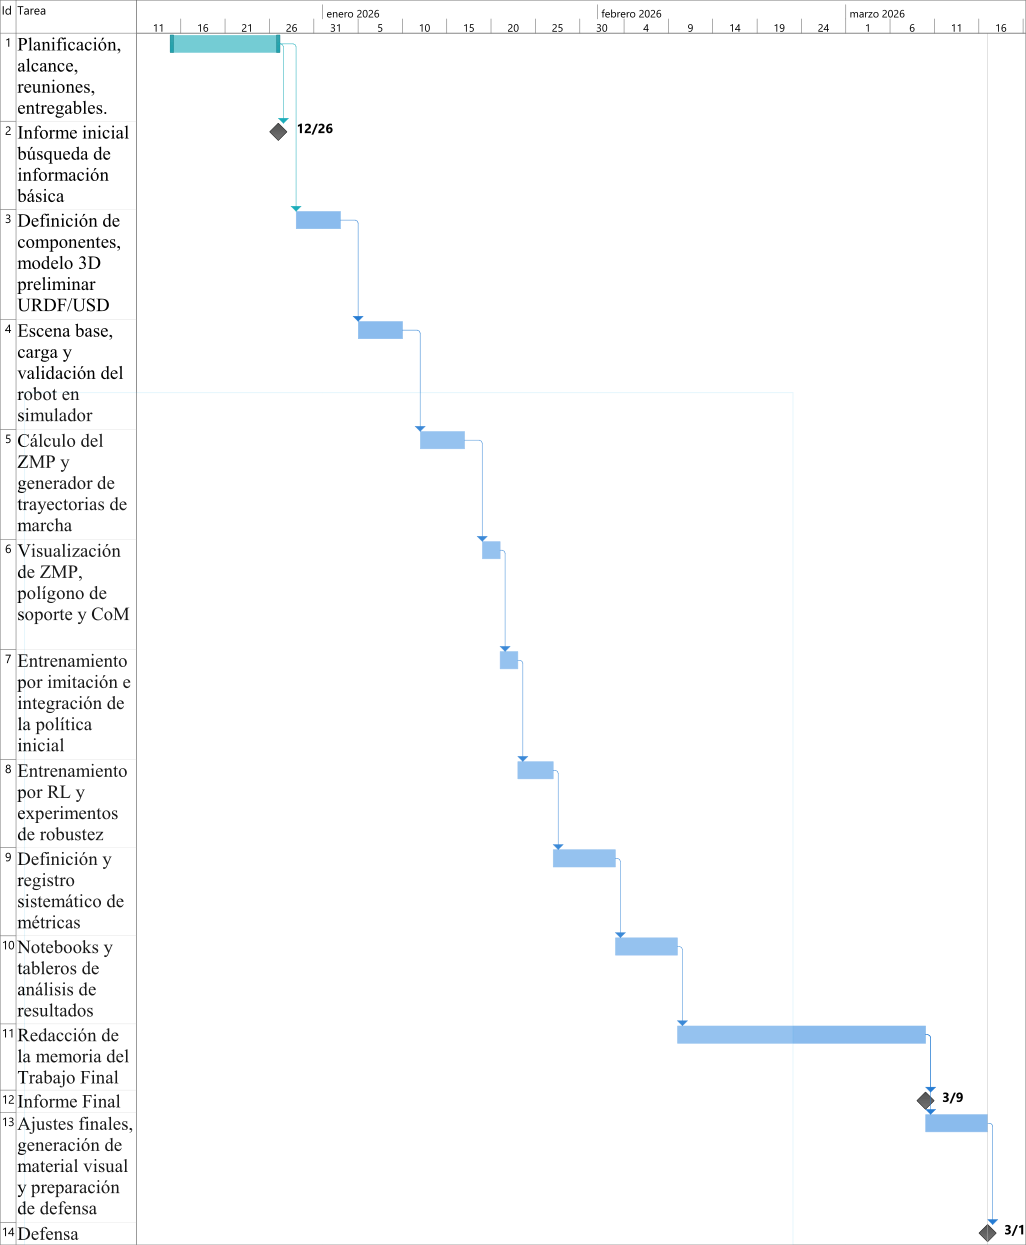
\includegraphics[width=1\textwidth]{./Figuras/gantt.png}
\caption{Diagrama de Gantt.}
%\label{fig:diagBloques}
\end{figure}


\section{12. Gobernanza de datos}
\label{sec:gobernanza}







No se capturan ni procesan datos personales de individuos ni información sensible; todo el comportamiento del agente se entrena sobre entornos sintéticos. El único material que se prevé publicar de forma abierta son el código fuente y las políticas entrenadas, junto con scripts de evaluación y documentación del experimento. 


\textbf{12.1. Cumplimiento normativo}



El simulador y los entornos asociados (NVIDIA Isaac Sim e Isaac Lab) se utilizarán bajo sus licencias de desarrollador, exclusivamente con fines académicos y no productivos. No se redistribuirán escenas ni assets propietarios.

Las bibliotecas de aprendizaje automático como PyTorch, frameworks de RL y arquitecturas tipo ResNet-18 se emplearán bajo sus licencias open source (BSD-3, MIT, Apache-2.0). En el repositorio del proyecto se incluirá un apartado con licencias y avisos correspondientes.



\textbf{12.2. Ética en el uso de inteligencia artificial}


El objetivo del proyecto es mejorar la autonomía de robots caminantes para tareas de construcción, un entorno en el que una caída o movimiento inapropiado podría implicar riesgos para personas y bienes. Este trabajo se desarrolla sólo en simulación: no se recomienda el uso de las políticas resultantes en robots físicos sin medidas de seguridad. Desde una perspectiva social, el proyecto busca automatizar tareas físicamente demandantes que son realizadas en entornos riesgosos. Al disminuir la exposición directa de los operarios a estas condiciones peligrosas, se contribuye significativamente a mejorar su seguridad. 


\section{13. Gestión de riesgos}
\label{sec:riesgos}



a) Identificación de los riesgos y estimación de sus consecuencias, con probabilidad y severidad graduadas de menor a mayor en escala de 1 a 10:
 
 
 
 
 
Riesgo 1: El robot bípedo no logra una marcha estable a pesar de las trayectorias generadas con ZMP, lo que podría impedir cumplir el objetivo principal del proyecto.

\begin{itemize}

	\item Severidad (S): 9. Si el robot no consigue caminar establemente, el propósito central del proyecto no se alcanzaría, por lo que el impacto sobre el proyecto es muy alto. .\\
	
	\item Probabilidad de ocurrencia (O): 5. Existe una probabilidad moderada, dado que la generación de
trayectorias con ZMP es compleja y podrían surgir factores imprevistos (como limitaciones del modelo o simplificaciones en la simulación) que dificulten la estabilidad.

\end{itemize}






 
Riesgo 2: El entrenamiento por Reinforcement Learning (RL) no converge o no mejora sustancialmente el andar obtenido por imitación, causando retrasos o resultados inferiores a lo
esperado.


\begin{itemize}

	\item Severidad (S): 8. Un bajo rendimiento de la fase de RL reduciría el valor del proyecto,
aunque el robot haya aprendido a caminar por imitación (el impacto es serio pero podría subsistir
un resultado parcial).\\

	\item Probabilidad de ocurrencia (O): 6. Es relativamente probable; los algoritmos de RL pueden requerir
muchos episodios y ajustes de hiperparámetros. Dado el tiempo limitado del proyecto y la
naturaleza estocástica del RL, existe riesgo de que la mejora sea más lenta de lo previsto.\\

	
\end{itemize}


 
Riesgo 3: Dificultades de integración entre los distintos módulos del proyecto (modelo 3D, cálculo de
ZMP, simulador, algoritmo de RL), provocando retrasos en el desarrollo.

\begin{itemize}

	\item Severidad (S): 6. Problemas de integración podrían detener el progreso temporalmente y requerir reprocesos, retrasando el avance del proyecto. Se espera que se puedan resolver con trabajo adicional.\\
	
	\item Probabilidad de ocurrencia (O): 7. Es bastante probable; integrar componentes de simulación,
control e IA se asocia a problemas como incompatibilidad de formatos y errores de comunicación entre herramientas.\\
	
	
\end{itemize}



 
Riesgo 4: Limitaciones de rendimiento o recursos de cómputo durante las simulaciones y entrenamientos, que impliquen tiempos de ejecución elevados o la necesidad de reducir el alcance del entrenamiento.

\begin{itemize}

	\item Severidad (S): 7. Si las simulaciones o entrenamientos toman demasiado tiempo, podría reducirse la
cantidad de experimentos y ajustes posibles, impactando la calidad de los resultados y la capacidad
de iteración.\\
	
	\item Probabilidad de ocurrencia (O): 6. Es probable en caso de usar entornos de simulación pesados o algoritmos complejos. Si no se puede usar la GPU local o no es suficiente ni se logra optimizar el proceso, el entrenamiento
podría volverse lento.\\
	
	
\end{itemize}




 
Riesgo 5: Calidad o cantidad insuficiente de datos de demostración generados con ZMP para el entrenamiento por imitación, lo que podría degradar el desempeño inicial de la política de control.

\begin{itemize}

	\item Severidad (S): 5. Un conjunto pobre de demostraciones podría llevar a una política inicial deficiente, aunque el agente luego podría mejorarse con RL. El impacto existe pero podría mitigarse en fases
posteriores.\\
	
	\item Probabilidad de ocurrencia (O): 4. Es moderadamente probable; depende del generador de ZMP. Si las trayectorias generadas no cubren suficientes variaciones o presentan errores, la calidad del dataset se verá comprometida.
\\
	
	
\end{itemize}




b) Tabla de gestión de riesgos: 

\begin{table}[htpb]
\centering
\begin{tabularx}{\linewidth}{@{}|X|c|c|c|c|c|c|@{}}
\hline
\rowcolor[HTML]{C0C0C0} 
Riesgo & S & O & RPN & S* & O* & RPN* \\ \hline
Que no se logre un andar estable a pesar de las trayectorias generadas con ZMP. & 9 & 5  &  45   &  9  &  3  &   27   \\ \hline
Que RL no mejore sustancialmente el andar obtenido por IL. & 8  & 6  &  48   &  6  & 4   &   24   \\ \hline
Dificultades de integración entre los distintos módulos del proyecto. & 6  &  7 &  42   &  6  &  3  &   18   \\ \hline
Insuficiente capacidad de cómputo durante las simulaciones y entrenamientos. &  7 & 6  &   42  &  7  &  4  &   28                                                                   \\ \hline
Insuficientes datos de demostración generados con ZMP para el entrenamiento por imitación. &  5 &  4 &  20   &    &    &      \\ \hline
\end{tabularx}%
\end{table}






Criterio adoptado: 

Se tomarán medidas de mitigación en los riesgos cuyos números de RPN sean mayores a 40.

Nota: los valores marcados con (*) en la tabla corresponden luego de haber aplicado la mitigación.

c) Plan de mitigación de los riesgos que originalmente excedían el RPN máximo establecido:
 
Riesgo 1: El agente no logra una marcha estable a pesar de las trayectorias generadas con ZMP.

  \begin{itemize}
	\item primero validar que el robot se mantenga de pie.
	\item simplificación del entorno inicial.
	\item Ajustar parámetros físicos del modelo según sea necesario y mantener consultas periódicas con el director para validar enfoques.
\end{itemize}




    

Nueva asignación de S y O:
\begin{itemize}
    \item Severidad (S*): 9. La severidad se mantiene alta porque, si el robot no logra una marcha estable, el objetivo principal del proyecto sigue comprometido.
    \item Probabilidad de ocurrencia (O*): 3. La probabilidad disminuye gracias al entorno en condiciones ideales, la validación temprana, ajustes de parámetros y consultas con el director.
\end{itemize}

 
 
 
 
 
Riesgo 2: RL no mejora sustancialmente el andar obtenido por IL.

Plan de mitigación:
\begin{itemize}    
    \item Reservar tiempo en el cronograma para ajuste de hiperparámetros y número suficiente de episodios, monitoreando métricas intermedias.
    \item Ajustar la función de recompensa, probar algoritmos de RL alternativos o simplificar el entorno de entrenamiento.
\end{itemize}


Nueva asignación de S y O:
\begin{itemize}

    \item Severidad (S*): 6. El proyecto mantiene resultados presentables incluso si RL no aporta grandes mejoras.
    \item Probabilidad de ocurrencia (O*): 4. Disminuye al dedicar más tiempo, monitoreo y flexibilidad para cambiar de algoritmo o configuración.
\end{itemize}


 
 


Riesgo 3: Dificultades de integración entre los distintos módulos del proyecto.

Plan de mitigación:
\begin{itemize}
    \item Integración continua y pruebas a medida que avanza el desarrollo.
    \item Atención al control de versiones sobre código, para poder identificar y revertir cambios.
    \item Utilizar formatos y herramientas estándar.
    \item Consultar documentación y foros.
\end{itemize}

Nueva asignación de S y O:
\begin{itemize}
    \item Severidad (S*): 6. Se mantiene igual, ya que un fallo de integración sigue implicando retrabajo relevante.
    \item Probabilidad de ocurrencia (O*): 3. Se reduce al detectar y corregir problemas de compatibilidad desde etapas tempranas.
\end{itemize}


 
 
 
Riesgo 4: Insuficiente capacidad de cómputo durante las simulaciones y entrenamientos.

Plan de mitigación:
\begin{itemize}
    \item Aumentar la capacidad de cómputo disponible.
    \item Programar entrenamientos ejecutarse durante la noche o fines de semana, aprovechando tiempo ocioso.
    \item Ajustar número de episodios para cumplir con el cronograma.
    \item Optimizar el entorno de simulación.
\end{itemize}

Nueva asignación de S y O:
\begin{itemize}
    \item Severidad (S*): 7. La severidad no cambia, ya que retrasos por recursos seguirían impactando el cronograma.
    \item Probabilidad de ocurrencia (O*): 4. Disminuye gracias a la mejor planificación de entrenamientos y el aumento de capacidad.
\end{itemize}



 





\section{14. Sprint Review}
\label{sec:sprint_review}


% \textbf{Tabla de revisión:}
\begin{table}[htpb]
\renewcommand{\arraystretch}{1.5}
\begin{tabular}{|>{\raggedright\arraybackslash}m{1.7cm}|
                >{\raggedright\arraybackslash}m{3.0cm}|
                >{\raggedright\arraybackslash}m{3cm}|
                >{\raggedright\arraybackslash}m{3cm}|
                >{\raggedright\arraybackslash}m{3cm}|}
\hline
\rowcolor[HTML]{CCCCCC}
\textbf{HU seleccionada} & \textbf{Tareas asociadas} & \textbf{Entregable esperado} & \textbf{¿Cómo sabrás que está cumplida?} & \textbf{Observaciones o riesgos} \\
\hline
                         & Determinar y especificar componentes, parámetros físicos y sensores. & Modelo 3D del robot integrado al entorno de simulación funcionando.                            &                 El modelo se exporta al simulador sin errores. 
                          &   Problemas de integración.                                  \\ \cline{2-2}
\multirow{-2}{=}{HU1}    & Modelo 3D con sensores, actuadores y vínculos. & \multirow{-2}{=}{} & \multirow{-2}{=}{Se comprueba que puede mantenerse en pie.} & \multirow{-2}{=}{} \\
\hline
                         & Implementar cálculo del ZMP a partir de fuerzas de contacto. &  Dataset sintético de trayectorias de marcha sin caídas.                           &             La herramienta genera N pasos de marcha sin que el robot caiga.                               &  Problemas en ajuste de parámetros                                   \\ \cline{2-2}
\multirow{-2}{=}{HU3}    & Implementar el generador de trayectorias de marcha basadas en ZMP. & \multirow{-2}{=}{} & \multirow{-2}{=}{} & \multirow{-2}{=}{} \\
\hline
                         & Entrenar la política inicial por imitación. &      Política de control de la marcha entrenada por imitación.                       &   El robot camina en el simulador con la nueva política.                                         &   Podría requerirse recopilar más demostraciones.                                  \\ \cline{2-2}
\multirow{-2}{=}{HU5}    & Integrar la política entrenada en el simulador y validar marcha básica. & \multirow{-2}{=}{} & \multirow{-2}{=}{Se cumplen los criterios de aceptación de estabilidad básica.} & \multirow{-2}{=}{} \\
\hline
                         & Configurar y ejecutar el algoritmo de RL. Entrenar en suelo irregular &   Política de control robusta entrenada con RL.                          &    El agente mantiene la marcha ante perturbaciones y cambios de velocidad.                                       &     Entrenamiento lento o necesidad de reajustar hiperparámetros.                                \\ \cline{2-2}
\multirow{-2}{=}{HU6}    &  y cambios de velocidad objetivo. & \multirow{-2}{=}{} & \multirow{-2}{=}{} & \multirow{-2}{=}{} \\
\hline
\end{tabular}
\end{table}

\section{15. Sprint Retrospective}    
\label{sec:sprint_retro}

En la siguiente tabla se sintetiza una primera aplicación de la Estrella de la Retrospectiva al proyecto. Para cada tipo de sprint se plantean prácticas a reforzar, hábitos a reducir, aspectos que conviene mantener y acciones nuevas a incorporar o abandonar. Esta esquematización ayuda a proponer ajustes concretos que faciliten el desarrollo del proyecto.


\begin{table}[htpb]
\renewcommand{\arraystretch}{1.3}
\begin{tabularx}{\linewidth}{@{}|X|X|X|X|X|X|@{}}
\hline
\rowcolor[HTML]{C0C0C0}
\textbf{Sprint tipo y N\textsuperscript{o}} &
\textbf{¿Qué hacer más?} &
\textbf{¿Qué hacer menos?} &
\textbf{¿Qué mantener?} &
\textbf{¿Qué empezar a hacer?} &
\textbf{¿Qué dejar de hacer?} \\
\hline
Sprint técnico 1
Modelo 3D y entorno &
Bloques de trabajo concentrado para avanzar en el modelo 3D y la configuración básica del simulador. &
Interrumpir el trabajo para probar herramientas nuevas que no son críticas para este sprint. &
Probar el modelo en escenas simples para validar colisiones y contactos antes de complejizar. &
Registrar en un log sencillo las decisiones de diseño y los problemas encontrados en cada sesión. &
Empezar tareas técnicas sin revisar antes el backlog y los criterios de aceptación asociados. \\
\hline
Sprint técnico 3
ZMP y trayectorias &
Ejecutar pruebas del cálculo de ZMP en patrón de marcha básico alternativo. &
Ajustar parámetros de forma improvisada sin comparar con resultados anteriores. &
Comparar las trayectorias obtenidas con el criterio teórico de estabilidad. &
Versionar scripts de prueba y gráficos en el repositorio para poder replicar experimentos. &
Modificar código directamente en el simulador sin guardar una versión previa. \\
\hline
Sprint técnico 6
Entrenamiento con RL &
Monitorear métricas de recompensa, caídas, energía en corridas largas de entrenamiento. &
Lanzar experimentos grandes sin pruebas preliminares en entornos reducidos. &
Usar semillas fijas y configuraciones documentadas para poder reproducir resultados. &
Planificar lotes pequeños de experimentos, cada uno con una hipótesis clara sobre el cambio a evaluar. &
Cambiar muchos hiperparámetros a la vez sin anotar qué se modificó ni qué se espera observar. \\
\hline
Sprint no técnico 9
Defensa &
Escribir breves resúmenes al cerrar cada bloque de trabajo técnico para facilitar la redacción. &
Dejar la escritura de secciones completas para los últimos días del sprint. &
Revisar la guía de formato antes de redactar apartados. &
Pedir feedback puntual sobre objetivos, resultados, conclusiones a una persona externa. &
Acumular correcciones en notas sueltas sin integrarlas periódicamente al documento principal. \\
\hline
\end{tabularx}
\end{table}













\end{document}